\documentclass[]{scrreprt}
\usepackage{amsmath,amsfonts,graphicx,tikz}

\def\species{\mathrm{sp}}
\def\phase{\mathrm{ph}}
\def\massfrac{\chi}
\def\flux{\mathbf{F}}
\def\darcyvel{\mathbf{v}}
\def\energydens{\mathcal{E}}
\def\d{\mathrm{d}}

\newcommand{\uo}{\mbox{UO\textsubscript{2}}\xspace}

\setcounter{secnumdepth}{3}


\begin{document}


\title{Broadbridge-White tests}
\author{CSIRO}
\maketitle

\tableofcontents


\chapter{The 2-phase analytic infiltration solution}
\label{bw}

The physical setup studied in this section is a 1D column that is
initially unsaturated, and which is subject to a constant injection of
fluid from its top.  This is of physical importance because it is a
model of constant rainfall recharge to an initially dry groundwater system.
The top surface becomes saturated, and this saturated zone moves
downwards into the column, diffusing as it goes.  The problem is of
computational interest because under certain conditions an analytic
solution is available for the saturation profile as a function of
depth and time.

The Richards' equation for an incompressible fluid in one
spatial dimension ($z$) reads
\begin{equation}
\dot{S} = \nabla \left(D \nabla S\right) - \nabla K \ ,
\end{equation}
where
\begin{eqnarray}
D(S) & = & -\frac{\kappa \kappa_{rel}}{\mu\phi}P_{\mathrm{c}}' \ ,
\\
K(S) & = &\frac{\rho g \kappa\kappa_{\mathrm{rel}}}{\mu\phi} \ .
\end{eqnarray}
Here $P_{\mathrm{c}} = -P$ which is the capillary pressure, and recall
that $P_{\mathrm{c}}'(S)<0$.

The analytic solution of this nonlinear diffusion-advection relevant
to constant infiltration to groundwater has been derived Broadbridge
and White\footnote{P Broadbridge, I White ``Constant rate rainfall
  infiltration: A versatile nonlinear model, 1 Analytical solution''.
  Water Resources Research 24 (1988) 145--154.} for certain functions
$D$ and $K$.   Broadbridge and White
assume the hydraulic conductivity is
\begin{equation}
K(S) = K_{n} + (K_{s}-K_{n})\frac{\Theta^{2}(C-1)}{C-\Theta} \ ,
\label{bw.krel}
\end{equation}
where
\begin{equation}
\Theta = \frac{S - S_{n}}{S_{s} - S_{s}} \ ,
\end{equation}
and the parameters obey $0 \leq K_{n} < K_{s}$, $0 \leq S_{n} \leq S
\leq S_{s}\leq 1$, and $C>1$.  The diffusivity is of the form
$a(b-S)^{-2}$.  This leads to very complicated relationships between
the capillary pressure, $P_{c}$, and the saturation, except in the
case where $K_{n}$ is small, when they are related through
\begin{equation}
\frac{P_{\mathrm{c}}}{\lambda_{s}} = \frac{\Theta - 1}{\Theta} - \frac{1}{C}\log
\left( \frac{C-\Theta}{(C-1)\Theta} \right) \ ,
\end{equation}
with $\lambda_{s}>0$ being the final parameter introduced by
Broadbridge and White.

Broadbridge and White derive time-dependent solutions for constant
recharge to one end of a semi-infinite line.  Their solutions are
quite lengthy, so I will not write them here.  To compare with MOOSE,
I use the following parameters --- the hydraulic parameters are those
used in Figure~3 of Broadbridge and White:
\begin{center}
\begin{tabular}{|ll|}
\hline
Bar length & 20\,m \\
Bar porosity & 0.25 \\
Bar permeability & 1 \\
\hline
Gravity & 0.1\,m.s$^{-2}$ \\
\hline
Fluid density & 10\,kg.m$^{-3}$ \\
Fluid viscosity & 4\,Pa.s \\
\hline
$S_{n}$ & 0\,m.s$^{-1}$ \\
$S_{s}$ & 1\,m.s$^{-1}$ \\
$K_{n}$ & 0\,m.s$^{-1}$ \\
$K_{s}$ & 1\,m.s$^{-1}$ \\
$C$ & 1.5 \\
$\lambda_{s}$ & 2\,Pa \\
\hline
Recharge rate $R_{\ast}$ & 0.5 \\
\hline
\end{tabular} \\
\end{center}
Broadbridge and white consider the case where the initial condition is
$S=S_{s}$, but this yields $P=-\infty$, which is impossible to use in
a MOOSE model.  Therefore the initial condition $P=-900$\,Pa is used
which avoids any underflow problems.  The recharge rate of
$R_{\ast}=0.5$ corresponds in the MOOSE model to a recharge rate of
$0.5\rho\phi(\kappa_{s}-\kappa_{n})=1.25$\,kg.m$^{-2}$.s$^{-1}$.  Note
that I've chosen $\frac{\rho g \kappa}{\mu \phi} = 1$\,m.s$^{-1}$, so
that the $K_{n}$ and $K_{s}$ may be encoded as $\kappa_{n}=0$ and
$\kappa_{s}=1$ in the relative permeability function
Eqn~(\ref{bw.krel}) in a straightforward way.

Figure~\ref{bw.fig} shows good agreement between the analytic solution
of Broadbridge and White and the MOOSE implementation.  There are
minor discrepancies for small values of saturation: these get smaller
as the temporal and spatial resolution is increased, but never totally
disappear due to the initial condition of $P=-900$\,Pa.

Two tests are part of the automatic test suite (one is marked
``heavy'' because it is a high-resolution version).

\begin{figure}[htb]
\centering
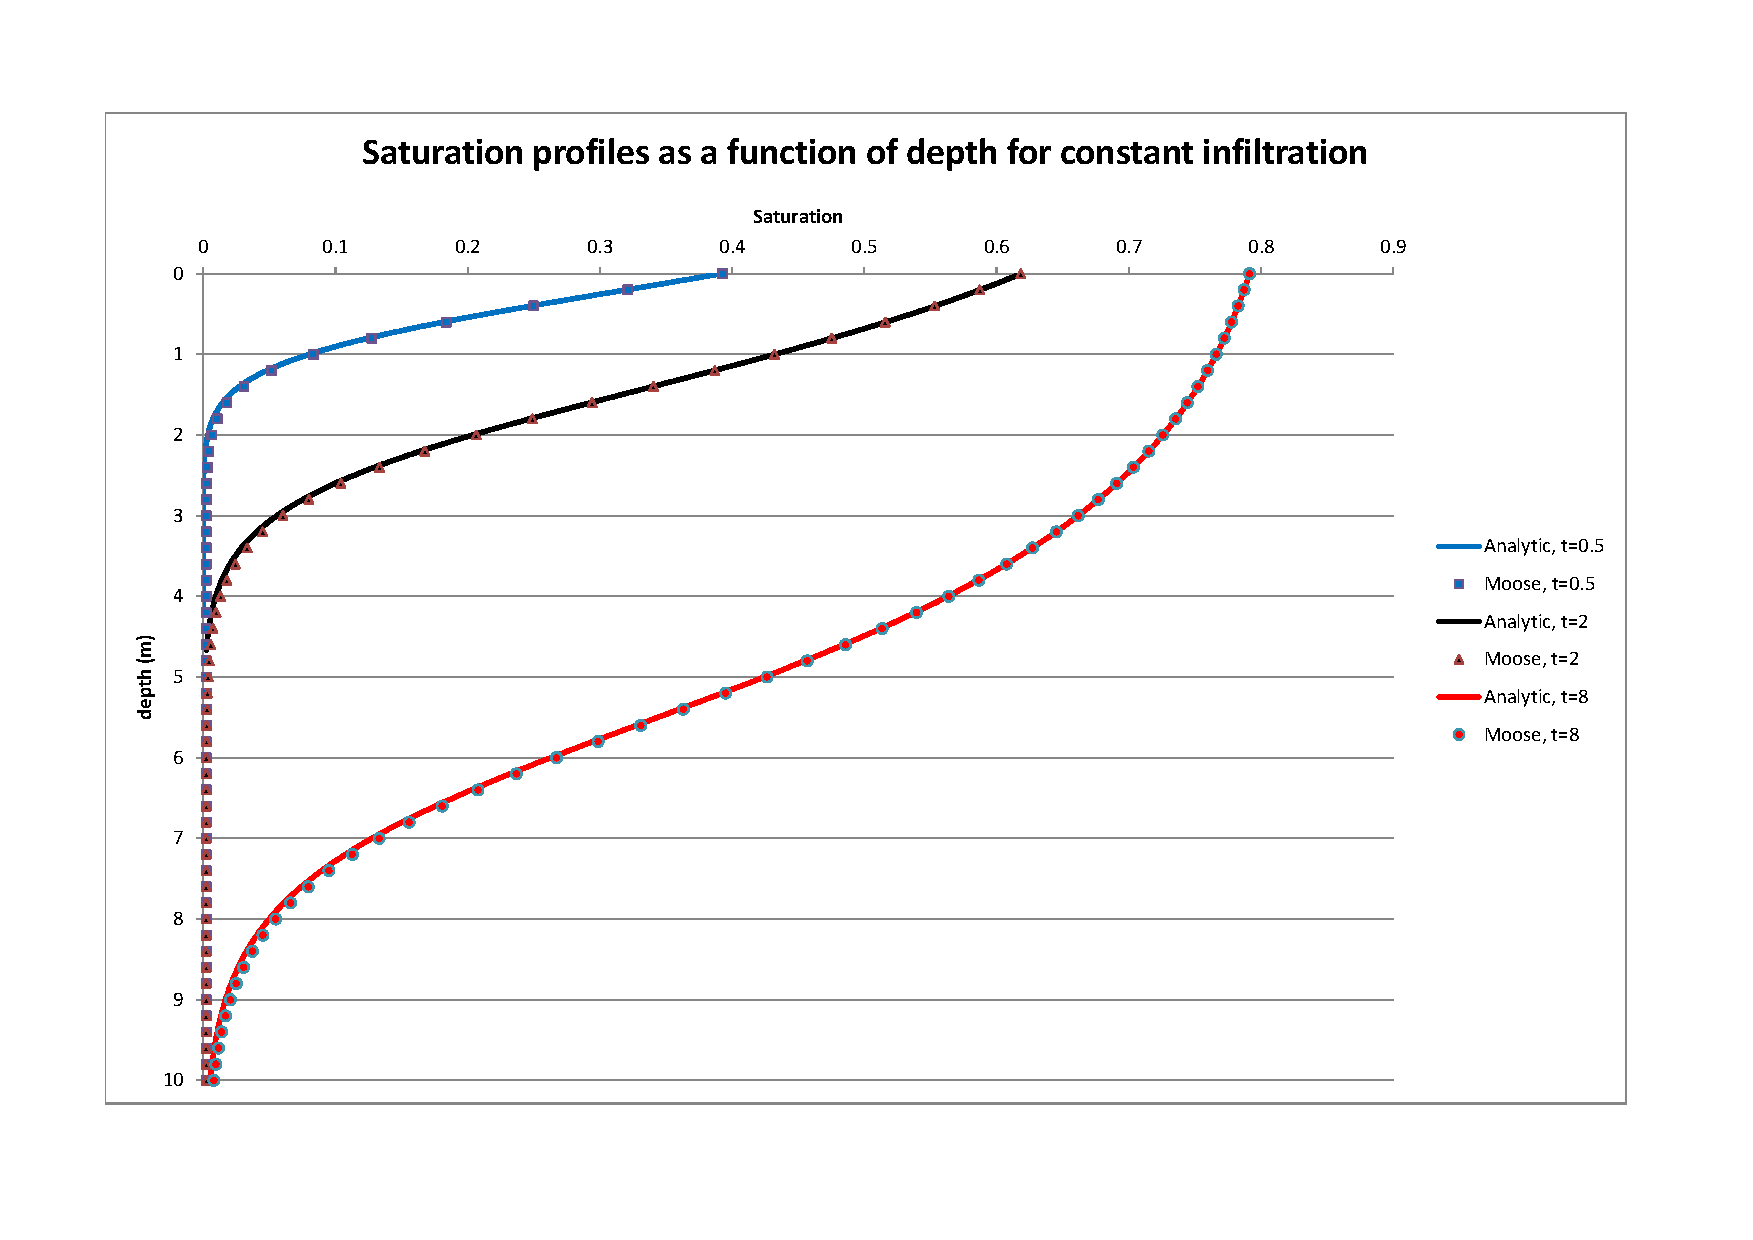
\includegraphics[width=16cm]{bw.pdf}
\caption{Comparison of the Broadbridge and White analytical solution
  with the MOOSE solution for 3 times.  This figure is shown in the
  standard format used in the Broadbridge-White paper: the constant
  recharge is applied to the $\mbox{depth}=0$ surface, and gravity
  acts downwards in this figure.}
\label{bw.fig}
\end{figure}


\chapter{The two-phase analytic drainage solution}
\label{wli}

Warrick, Lomen and Islas\footnote{AW Warrick, DO Lomen and A Islas,
  ``An analytical solution to Richards' Equation for a Draining Soil
  Profile'', Water Resources Research 26 (1990) 253--258.} extended
the analysis of Broadbridge and White (Chapter~\ref{bw}) to include
the case of drainage from a medium.

The setup is an initially-saturated infinitely-long column of material
that drains freely from its lower end.  This is simulated by placing a
boundary condition of $P=0$ at the lower end.  To obtain their analytical
solutions, Warrick, Lomen and Islas make the same assumptions as
Broadbridge and White concerning the diffusivity and conductivity of
the medium.  Their solutions are quite lengthy, so I will not write
them here.

A MOOSE model with the parameters almost identical to those listed in
Chapter~\ref{bw} is compared with the analytical solutions.  The only
differences are that the ``bar'' length is 10000\,m (to avoid any
interference from the lower Dirichlet boundary condition), and
$R_{\ast}=0$ since there is no recharge.  The initial condition is
$P=10^{-4}$\,Pa: the choice $P=0$ leads to poor convergence since
by construction the Broadbridge-White capillary function is only
designed to simulate the unsaturated zone $P<0$ and a sensible
extension to $P\geq 0$ is discontinuous at $P=0$.

Figure~\ref{wli.fig} shows good agreement between the analytic
solution and the MOOSE implementation.  Any minor discrepancies get
smaller as the temporal and spatial resolution increase.

This test is part of the automatic test suite that is run every time
the code is updated.


\begin{figure}[htb]
\centering
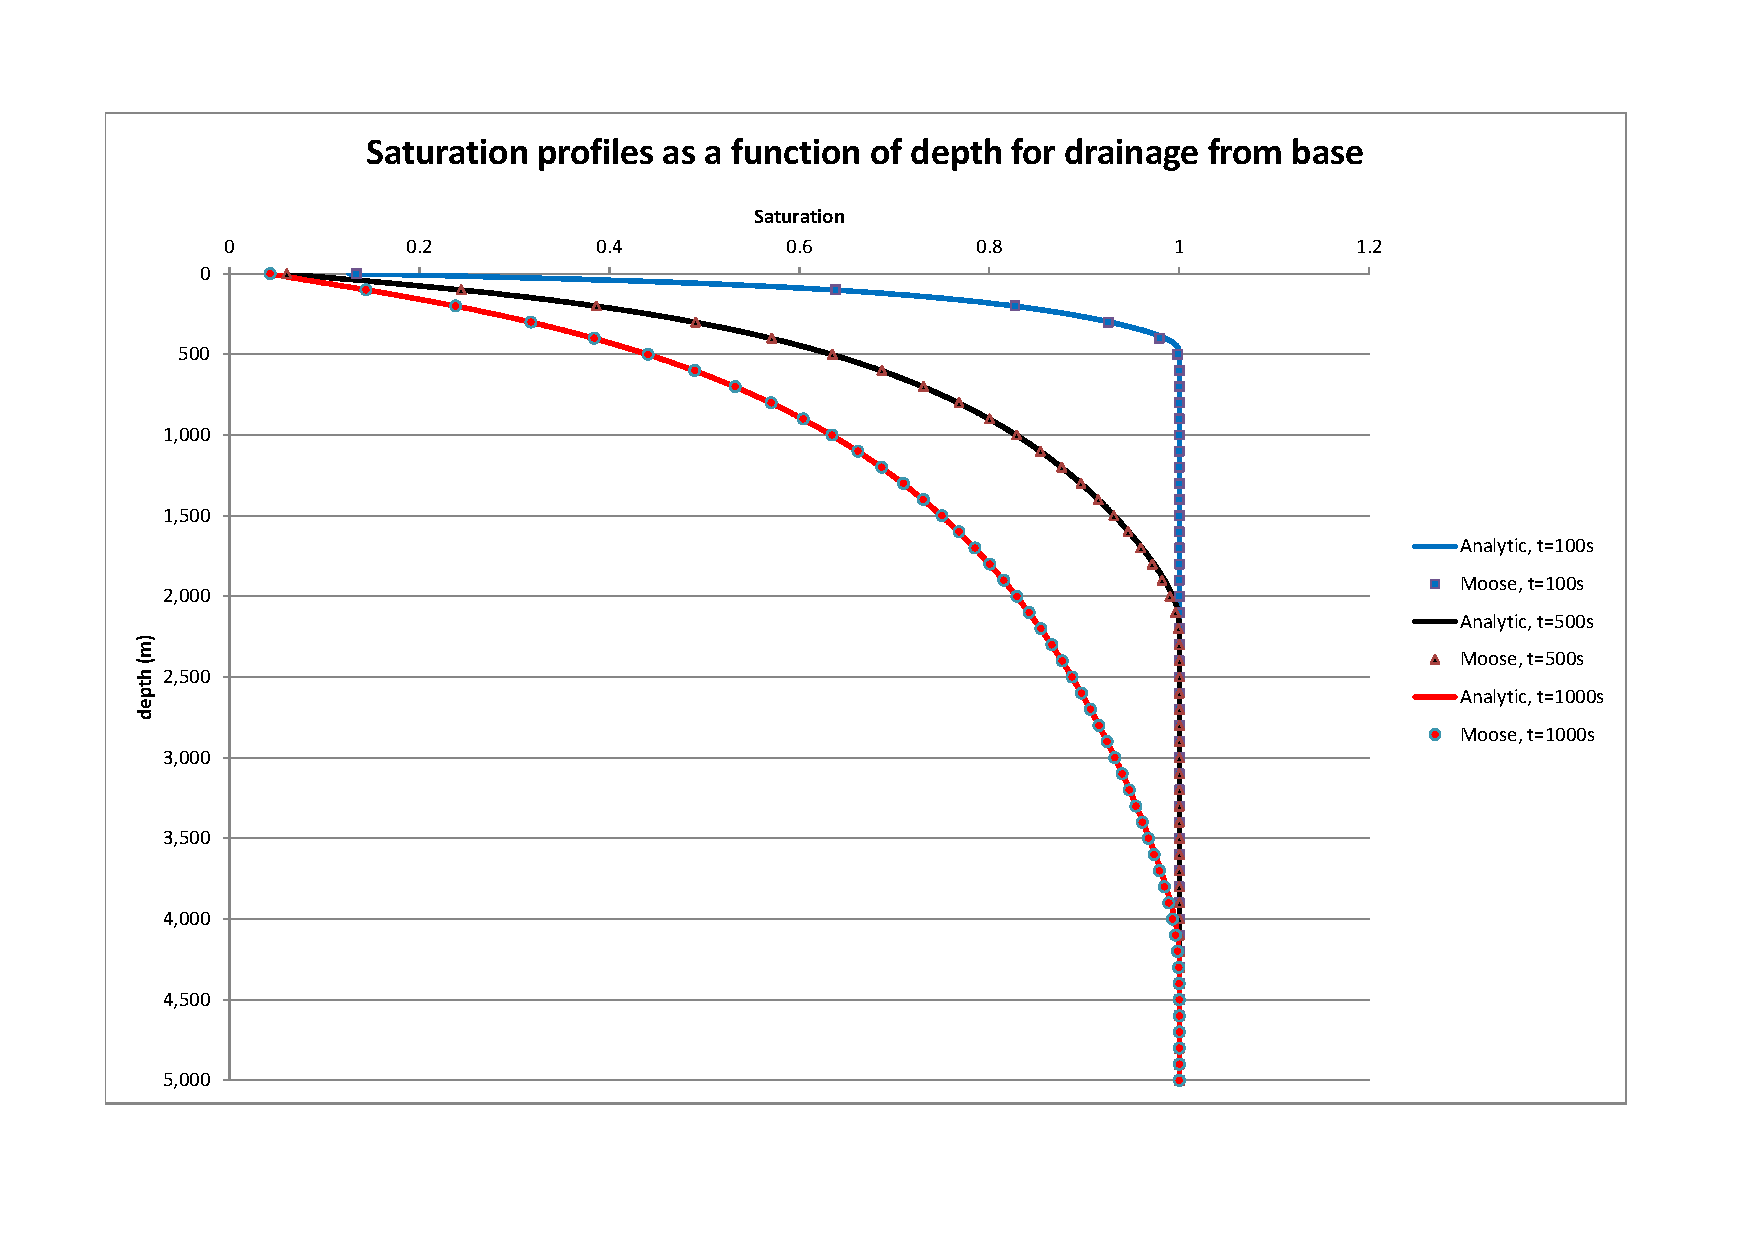
\includegraphics[width=16cm]{wli.pdf}
\caption{Comparison of the Warrick, Lomen and Islas analytical solution
  with the MOOSE solution for 3 times.  This figure is shown in the
  standard format used in the literature: the top of the model is
  $\mbox{depth}=0$ surface, and gravity acts downwards in this figure,
with fluid draining from $\mbox{depth}=\infty$.}
\label{wli.fig}
\end{figure}



\chapter{Single-phase infiltration and drainage}
\label{forsyth}

Forsyth, Wu and Pruess\footnote{PA Forsyth, YS Wu and K Pruess,
  ``Robust numerical methods for saturated-unsaturated flow with dry
  initial conditions in heterogeneous media'', Advances in Water
  Resources 18 (1995) 25--38} describe a HYDRUS simulation of an
experiment involving infiltration (experiment 1) and subsequent
drainage (experiment 2) in a large caisson.  The simulation is
effectively one dimensional, and is shown in
Figure~\ref{rd_setup.fig}.

\begin{figure}[htb]
\begin{center}
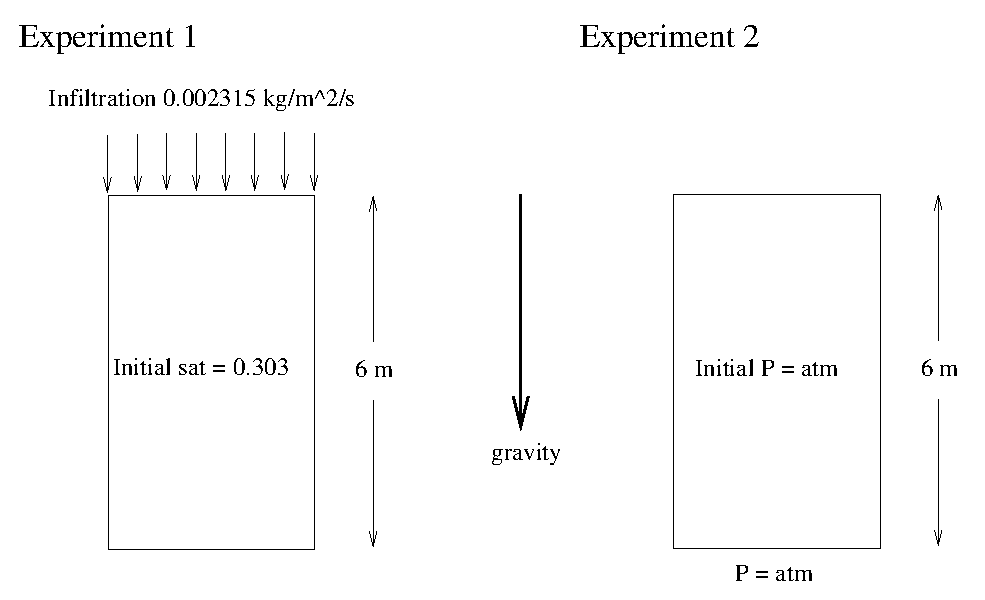
\includegraphics[width=12cm]{rd_setup.eps}
\caption{Two experimental setups from Forsyth, Wu and Pruess.
  Experiment 1 involves infiltration of water into an initially
  unsaturated caisson.  Experiment 2 involves drainage of water from
  an initially saturated caisson.}
\label{rd_setup.fig}
\end{center}
\end{figure}

The properties common to each experiment
are:
\begin{center}
\begin{tabular}{|ll|}
\hline
Caisson & 0.33 \\
Caisson permeability & $2.95\times 10^{-13}$\,m$^{2}$ \\
\hline
Gravity & 10\,m.s$^{-2}$ \\
\hline
Water density & 1000\,kg.m$^{-3}$ \\
Water viscosity & 0.00101\,Pa.s \\
Water bulk modulus & 20\,MPa \\
Water residual saturation & 0.0 \\
Air residual saturation & 0.0 \\
Air pressure & 0.0 \\
\hline
van Genuchten $\alpha$ & $1.43\times 10^{-4}$\,Pa$^{-1}$ \\
van Genuchten $m$ & 0.336 \\
van Genuchten turnover & 0.99 \\
\hline
\end{tabular} \\
\end{center}
In each experiment 120 finite elements were used along the length of
the Caisson.  The modified van-Genuchten relative permeability curve
with a ``turnover'' (set at $S=0.99$) was employed in order to improve
convergence significantly.  Hydrus also uses a modified van-Genuchten
curve, although I couldn't find any details on the modification.

In experiment 1, the caisson is initially at saturation 0.303
($P=-72620.4$\,Pa), and water is pumped into the top with a rate
0.002315\,kg.m$^{-2}$.s$^{-1}$.  This causes a front of water to
advance down the caisson.  Figure~\ref{rd.result.fig} shows the
agreement between MOOSE and the published result (this result was
obtained by extracting data by hand from online graphics).

In experiment 2, the caisson is initially fully saturated at $P=0$,
and the bottom is held at $P=0$ to cause water to drain via the action
of gravity.  Figure~\ref{rd.result.fig} shows the agreement between
MOOSE and the published result.

Experiment 1 and the first 4 simulation days of experiment 2 are
marked as ``heavy'' in the PorousFlow test suite since the simulations
take around 3 seconds to complete.  This means they are not run by
default every time the code is updated, and must be run manually.
However, the final 96 days of experiment 2 run quickly and are part of
the automatic test suite.


\begin{figure}[htb]
\begin{center}
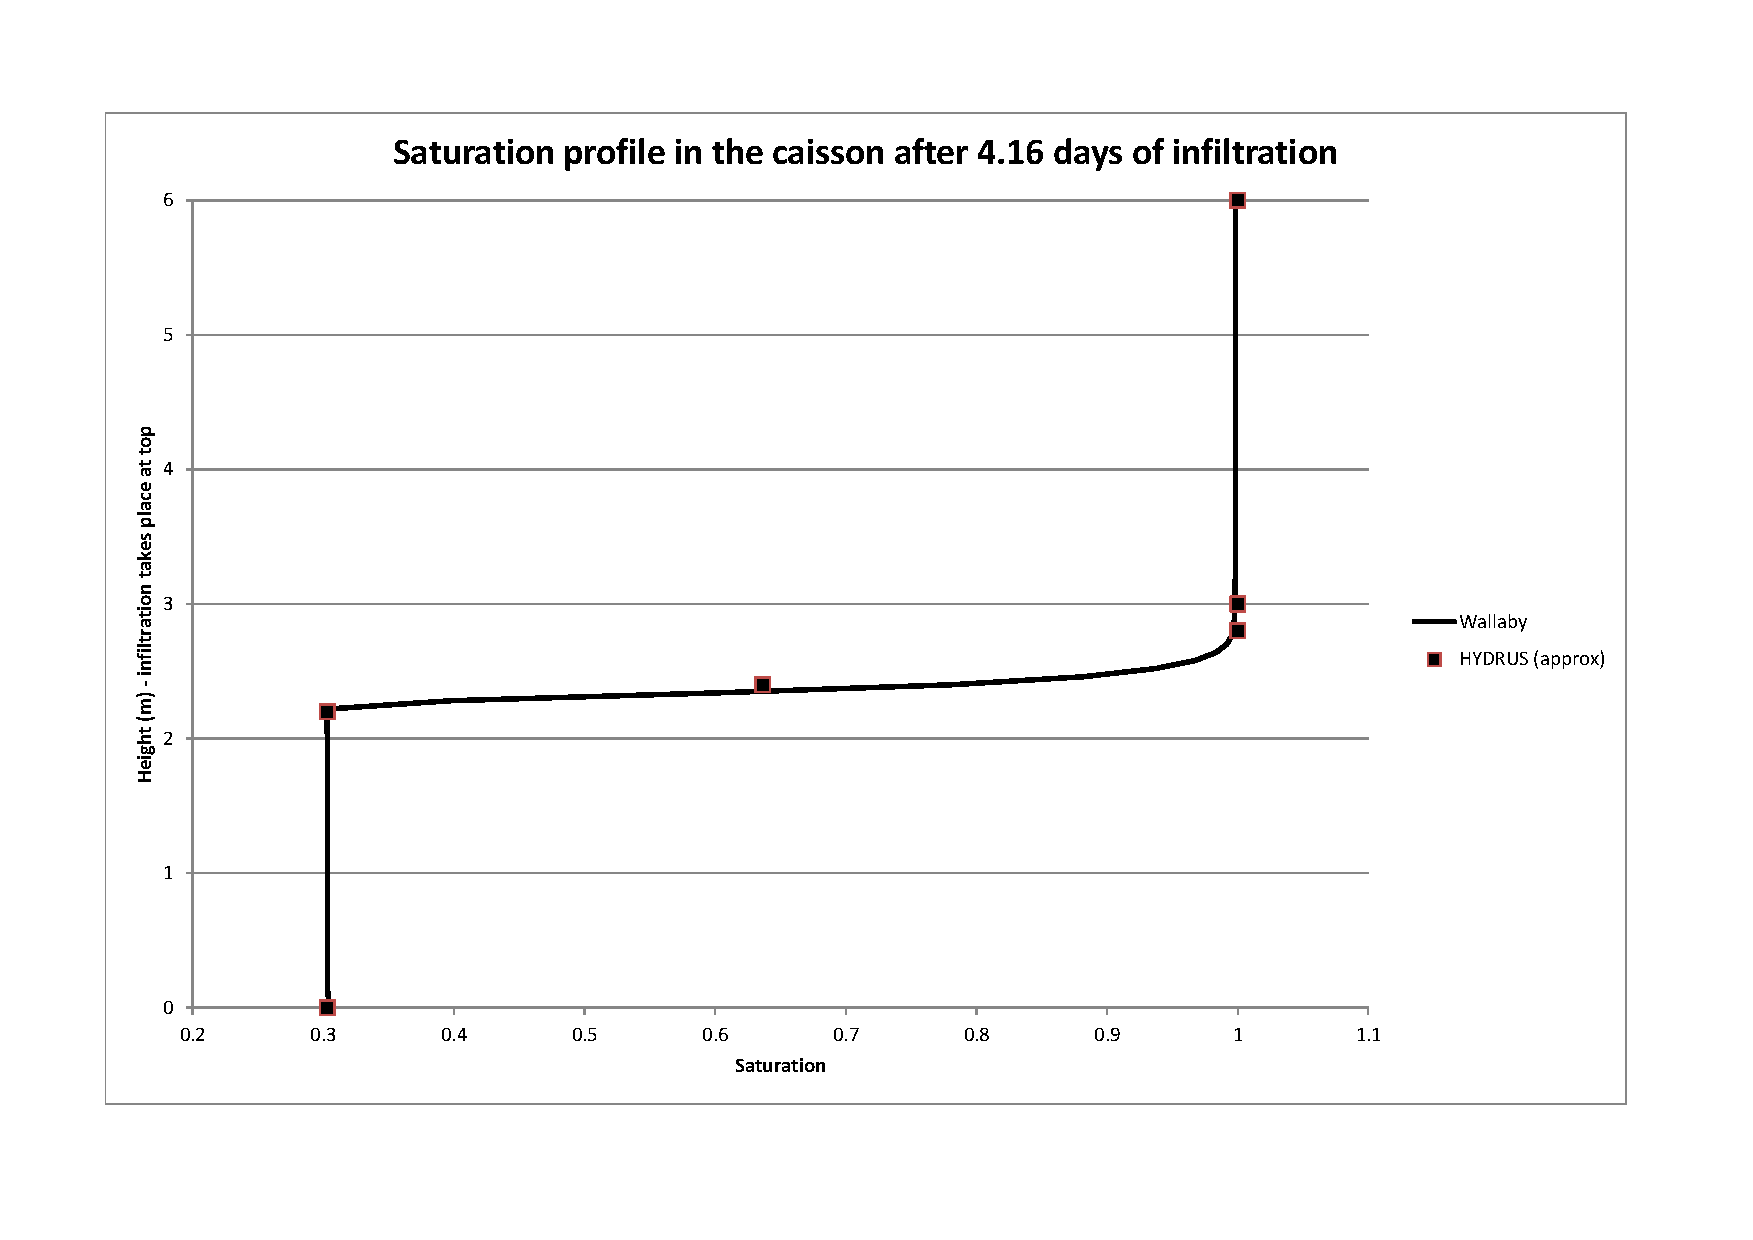
\includegraphics[width=12cm]{rd01.pdf} \\
$\mbox{}$\\
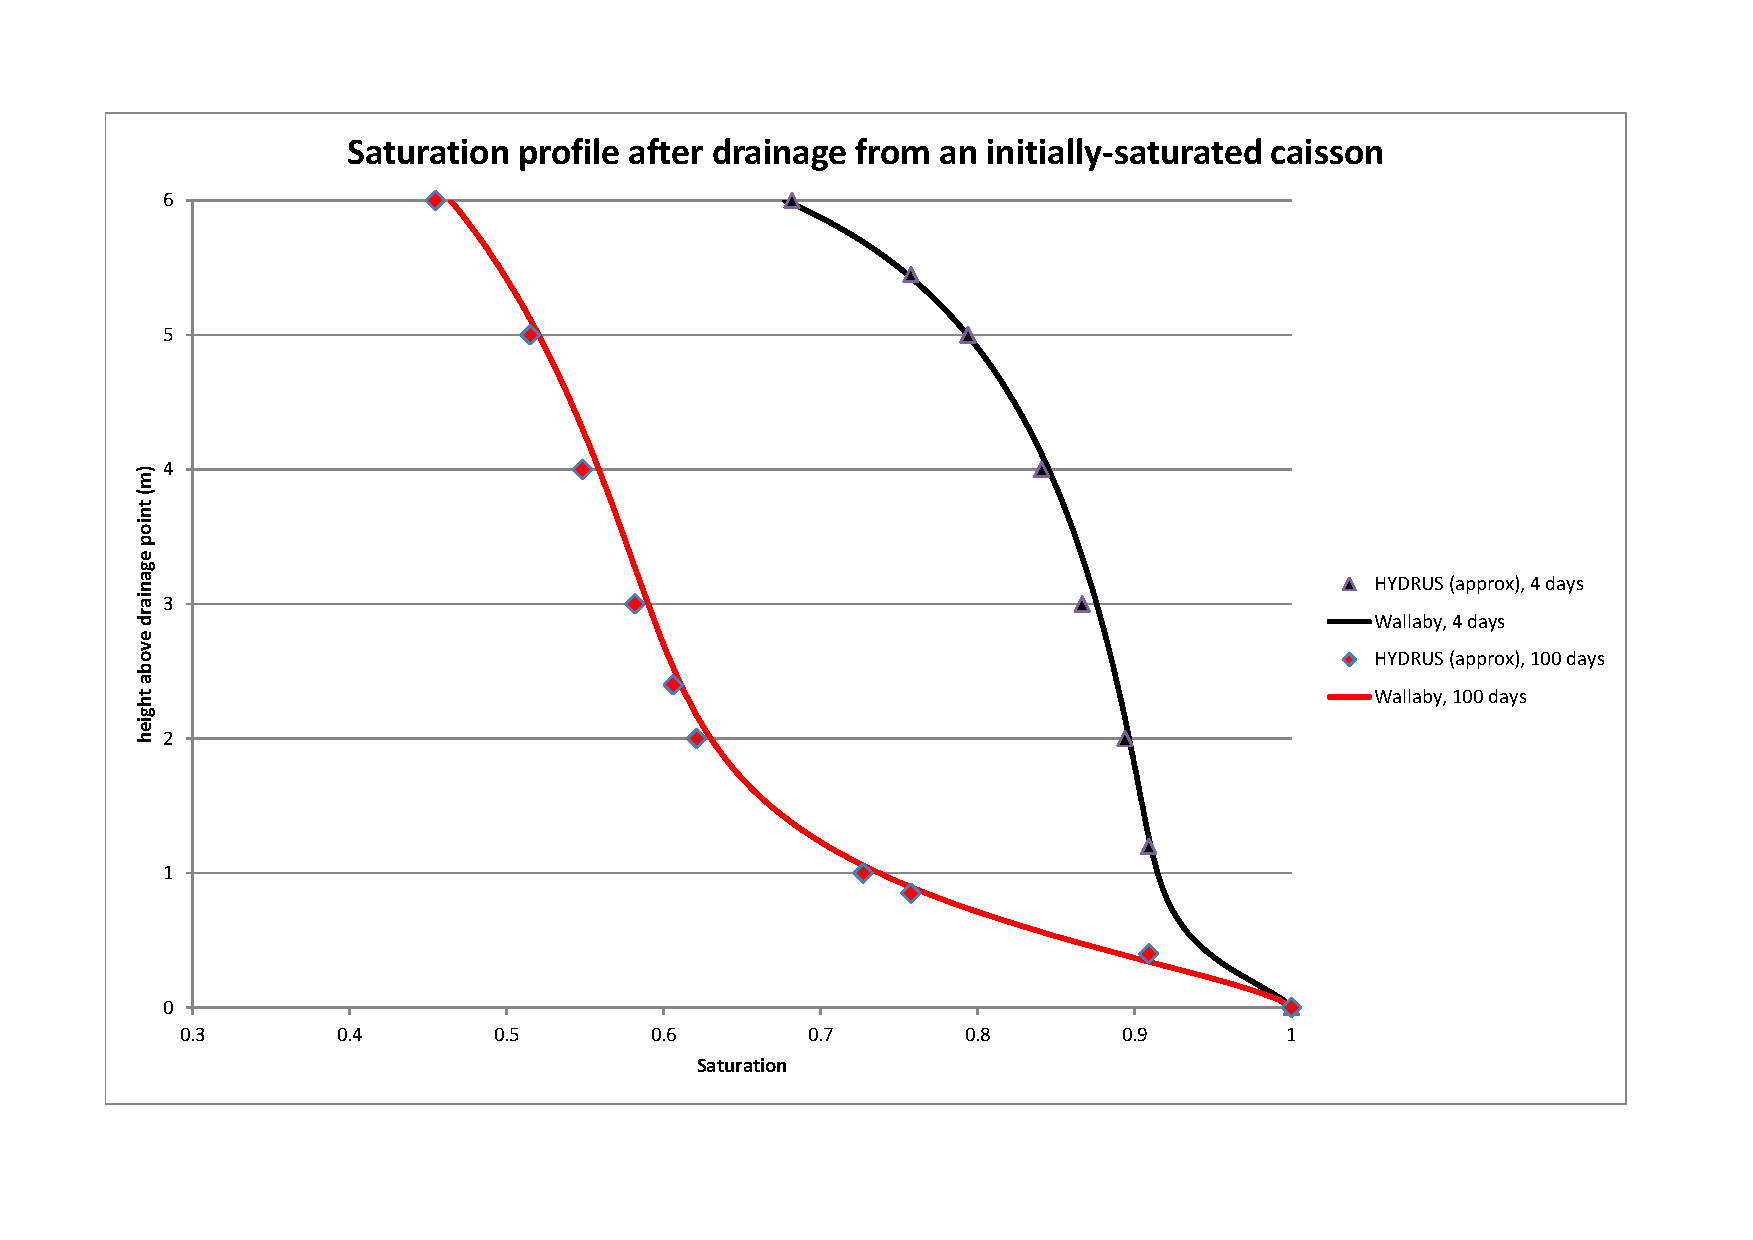
\includegraphics[width=12cm]{rd02.pdf}
\caption{Saturation profiles in the caisson.  Top: After 4.16 days of
  infiltration.  Bottom: After drainage from an initially-saturated
  simulation (4 days and 100 days profiles).  Note that the HYDRUS
  results are only approximate as I extrated the data by hand from
  online graphics.}
\label{rd.result.fig}
\end{center}
\end{figure}


\end{document}
